\documentclass[a4paper]{article}
\usepackage{graphicx}
\usepackage{siunitx}
\usepackage{csvsimple}
\usepackage{multirow}
\usepackage{booktabs}
\usepackage{amsmath,amsfonts,mathtools}
\usepackage[margin=3cm]{geometry}
\usepackage[bottom]{footmisc}

    \begin{document}
        \section{Implementation of Flip-Flop D and SR Latch with discrete logic gates}
        Using the schematic on Figure \ref{fig:Schem} the logic gates were implemented on a PCB.
        
        \begin{figure}[h!]
            \begin{center}
                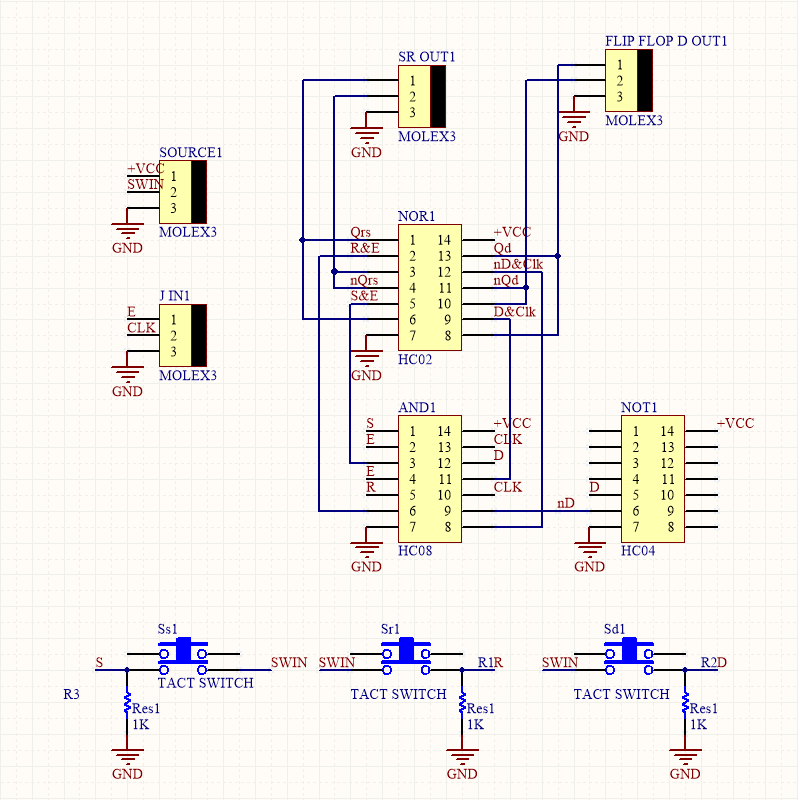
\includegraphics[width=\linewidth]{e6Schem.png}
                \caption{Schematic of the  SR Latch (on the left) and Flip-Flop D (on the right)}
            \end{center}
            \label{fig:Schem}
        \end{figure}

        The resulting circuits were tested and compared to their resulting counterparts as shown in
        Table \ref{tab:e6t1} and Table \ref{tab:e6t2}.

        \begin{table}[ht]
            \begin{center}
                \begin{tabular}{|l|l|r|r|r|r|r|r|c|}
    \toprule
    Symbol  &Parameter  &\multicolumn{3}{c|}{SN54279}&\multicolumn{3}{c|}{Experimental}&Unit\\
            &           &   MIN&N/T&MAX&MIN&N/T&MAX&\\
    \midrule
    $V_{CC}$&Supply Voltage&4.75&5&5.25&0.7&5&$?$&V\\
    $V_{IH}$&High-level input voltage&2&$-$&$-$&3.79&$-$&$-$&V\\
    $V_{IL}$&Low-level input voltage&$-$&$-$&0.8&$-$&$-$&1.35\footnote{This was assumed from the corresponding value for the 74HC08}&V\\
    \midrule
    $V_{OH}$&High-level output voltage&2.4&3.4&$-$&3.88&5&$-$&V\\
    $V_{OL}$&Low-level output voltage &$-$&0.2&0.4&$-$&0&0.06&V\\
    \midrule
    $t_{pHL}$&Phase Difference&$-$&9&15&$-$&$-$&10&ns\\
    $t_{pLH}$&Phase Difference&$-$&12&22&$-$&$-$&20&ns\\
    \bottomrule
\end{tabular}
\caption{Comparison of measured circuit characteristics for the Latch SR}
                \label{tab:e6t1}
            \end{center}
        \end{table}
        \begin{table}[ht]
            \begin{center}
                \begin{tabular}{|l|l|r|r|r|r|r|r|c|}
    \toprule
    Symbol  &Parameter  &\multicolumn{3}{c|}{74HC74}&\multicolumn{3}{c|}{Experimental}&Unit\\
            &           &   MIN&NOM&MAX&MIN&NOM&MAX&\\
    \midrule
    $V_{CC}$&Supply Voltage&2&5&6&1.5&5&$?$&V\\
    $V_{IH}$&High-level input voltage&3.15&$-$&$-$&2.64&$-$&$-$&V\\
    $V_{IL}$&Low-level input voltage&$-$&$-$&1.35&$-$&$-$&2.57&V\\
    $V_{I}$ &Input voltage&0&$-$&$V_{CC}$&0&$-$&$V_{CC}$&V\\
    $V_{O}$ &Output voltage&0&$-$&$V_{CC}$&-0.2&$-$&$V_{CC}$&V\\
    $\Delta t / \Delta v$&  Input rise and fall time&$-$&$-$&0.5&$-$&$-$&16.05&$\mu$s\\
    \midrule
    $V_{OH}$&High-level output voltage&3.84&4.3&$-$&3,725&$V_{CC}$&$-$&V\\
    $V_{OL}$&Low-level output voltage &$-$&0.17&0.4&$-$&-0.2&1.09&V\\
    \midrule
    $t_{pd}$&Phase Difference&$-$&20&44&$-$&28&56&ns\\  %Revise
    \bottomrule
\end{tabular}
\caption{Comparison of measured circuit characteristics for the Flip-Flop D}
                \label{tab:e6t2}
            \end{center}
        \end{table}
        
        First, in Table \ref{tab:e6t1} we can see that the operating conditions of the circuit are vastly different:
        We can see that, for example, $V_{CC}$ has a wider operating range in the experimental circuit than the Integrated
        circuit it is compared to. The fact that the fabricated circuit was made from more modern components than the SN54279
        might account for this difference in operating conditions. On the other hand, the phase differences are fairly similar
        for both circuits.

        Second, in Table \ref{tab:e6t2} there are notable differences on the characteristics of the circuit:
        the operating voltages are clearly different from those of its commercial counterpart, and the
        delays between the input and output signals are significantly higher. Given that the fabricated device
        has wires between each logic gate, it is expected that signals would take longer to travel between each
        component; therefore, the delay between the input signal and the output signal will be longer in the
        experimental circuit than in an Integrated Circuit.

        From the differences observed in both devices, one can conclude that both experimentally fabricated devices can
        be used interchangeably with their commercially available counterparts as long as they are not used in highly time-sensitive
        conditions. Otherwise, when one is working with signals at the order of $MHz$ it is adviced to use the commercially available
        equivalents.
    \end{document}